\documentclass[11pt, letterpaper]{article}
\usepackage[margin=1in]{geometry}
\usepackage{fancyhdr}
\usepackage[T1]{fontenc}
\usepackage{tabularx}
\usepackage{graphicx}
\usepackage{amssymb}
\usepackage[table, dvipsnames]{xcolor}
\usepackage{tikz}
\usepackage{tabularx}

\let\oldemptyset\emptyset
\let\emptyset\varnothing

\pagestyle{fancy}
\renewcommand{\headrulewidth}{0pt}

\fancyhf{}
\fancyfoot[R]{\thepage}

\graphicspath{ {./images/} }

\begin{document}

\noindent Riley Rice (riceri@oregonstate.edu)\\CS321\\12-2-2024

\begin{center}\noindent {\Huge \textbf{Homework 5}}\end{center}

\section*{Problem 1: [10 points]}

\noindent For each of the following statements, decide whether it is true or false. If true, write a letter "T"; if false, write a letter "F". Either way, also give a brief explanation (1-3 sentences).

\vspace{2mm}

\noindent\textbf{Hint:} Do not forgot to include the explanations...

\vspace{5mm}

\noindent \textbf{(a) Let the alphabet $\sum = \{a, b\}$. The regular expressions $(a^*b)^*a^*$ and $(a + b)^*$ represent the same language.}

\vspace{2mm}

\noindent\textbf{Answer:} True

\noindent \textbf{Explanation:} The regular expression $(a^*b)^*a^*$ generates all strings consisting of $a$s and $b$s, as $a^*$ represents zero or more $a$s, and $b$ appears in between as needed. Similarly, $(a+b)^*$ represents all strings over $\{a,b\}$. Since both generate the same set of strings, they represent the same language.

\vspace{5mm}

\noindent \textbf{(b) The CFG:} 

\vspace{2mm}

\textbf{$S \rightarrow aSb|bSa|a|b|\epsilon$}

\vspace{2mm}

\noindent \textbf{Decides the language $\{w \in \{a, b\}^*$ | $w$ is a palindrome$\}$}

\vspace{2mm}

\noindent\textbf{Answer:} True

\noindent \textbf{Explanation:} This CFG generates palindromes over the alphabet $\sum = \{a,b\}$. The rules $aSb$ and $bSa$ ensure that the string begins and ends with matching symbols, while the terminal rules $a$, $b$, and $\epsilon$ handle single characters and the empty string. Therefore, the CFG correctly defines the language of palindromes.

\vspace{5mm}

\noindent \textbf{(c) Let the alphabet $\sum = \{a\}$. There exists a DFA with only two states that decide the language $\{a\}$, i.e., the set of a single string "$a$". (Note that the problem mentions a DFA, not an NFA.)}

\vspace{2mm}

\noindent\textbf{Answer:} False

\noindent \textbf{Explanation:} A DFA for the language $\{a\}$ requires three states: one start state, one accepting state for a single $a$, and one trap state for inputs longer than or different from $a$. With only two states, the DFA cannot distinguish between strings of different lengths or handle invalid inputs correctly.

\vspace{5mm}

\noindent \textbf{(d) Let the alphabet $\sum = \{a\}$. There exists a Turing machine that decides the language $\{a^n$ | $n$ is a multiple of 3$\}$.}

\vspace{2mm}

\noindent\textbf{Answer:} True

\noindent \textbf{Explanation:} A Turing machine can decide this language by counting the number of $a$s modulo 3. It can move through the input tape, marking every third $a$ as it counts. If the tape ends exactly after marking a multiple of three $a$s, it accepts; otherwise, it rejects. This process is within the capability of a Turing machine.

\vspace{5mm}

\noindent \textbf{(e) In the execution of a Turing machine, once it enters an accepting state, the execution halts.}

\vspace{2mm}

\noindent\textbf{Answer:} True

\noindent \textbf{Explanation:} The Turing machine halts once it reaches an accepting or rejecting state. Although the TM may never halt if for example it has an infinite loop.

\newpage

\section*{Problem 2: [10 points]}

\noindent \textbf{(b):} Let the alphabet $\sum = \{a, b\}$. Construct a Turing machine that decides the language $L = \{w $| w contains an even number of $a$s and an even number of $b$s$\}$. (For example, $aaaaaa$, $abaaab$ and $\epsilon$ are in $L$, while $abbaa$ is not.) Your Turing machine must be in the form of a table similar to the examples in lectures 23 and 24; in particular, do not draw a transition graph.

\vspace{5mm}

\noindent \textbf{Hint:} $L$ is actually a regular language, and it's not too hard to come up with a DFA that decides it. Then turn this DFA into a Turing machine. The answer should be much simpler than the Turing machines we saw in class. Make sure that the format is correct (whenever in doubt, check lectures 23 and 24).
\vspace{5mm}

\noindent\textbf{Solution:}

\vspace{5mm}

\noindent Equivalent DFA:

\begin{center}
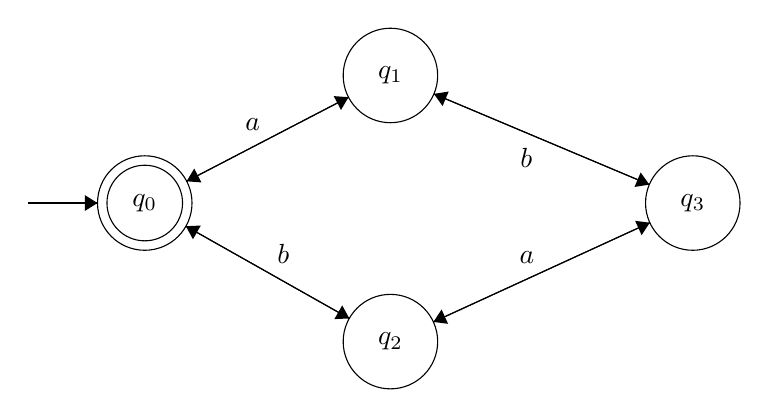
\begin{tikzpicture}[scale=0.2]
\tikzstyle{every node}+=[inner sep=0pt]
\draw [black] (7.6,-11.4) circle (3);
\draw (7.6,-11.4) node {$q_0$};
\draw [black] (7.6,-11.4) circle (2.4);
\draw [black] (23.2,-3.3) circle (3);
\draw (23.2,-3.3) node {$q_1$};
\draw [black] (42.4,-11.4) circle (3);
\draw (42.4,-11.4) node {$q_3$};
\draw [black] (23.2,-20.2) circle (3);
\draw (23.2,-20.2) node {$q_2$};
\draw [black] (0.2,-11.4) -- (4.6,-11.4);
\fill [black] (4.6,-11.4) -- (3.8,-10.9) -- (3.8,-11.9);
\draw [black] (10.26,-10.02) -- (20.54,-4.68);
\fill [black] (20.54,-4.68) -- (19.6,-4.61) -- (20.06,-5.49);
\draw [black] (20.54,-4.68) -- (10.26,-10.02);
\fill [black] (10.26,-10.02) -- (11.2,-10.09) -- (10.74,-9.21);
\draw (14.46,-6.85) node [above] {$a$};
\draw [black] (25.96,-4.47) -- (39.64,-10.23);
\fill [black] (39.64,-10.23) -- (39.09,-9.46) -- (38.7,-10.38);
\draw (31.83,-7.86) node [below] {$b$};
\draw [black] (39.64,-10.23) -- (25.96,-4.47);
\fill [black] (25.96,-4.47) -- (26.51,-5.24) -- (26.9,-4.32);
\draw [black] (25.93,-18.95) -- (39.67,-12.65);
\fill [black] (39.67,-12.65) -- (38.74,-12.53) -- (39.15,-13.44);
\draw [black] (39.67,-12.65) -- (25.93,-18.95);
\fill [black] (25.93,-18.95) -- (26.86,-19.07) -- (26.45,-18.16);
\draw (31.87,-15.29) node [above] {$a$};
\draw [black] (20.59,-18.73) -- (10.21,-12.87);
\fill [black] (10.21,-12.87) -- (10.66,-13.7) -- (11.16,-12.83);
\draw (16.4,-15.3) node [above] {$b$};
\draw [black] (10.21,-12.87) -- (20.59,-18.73);
\fill [black] (20.59,-18.73) -- (20.14,-17.9) -- (19.64,-18.77);
\end{tikzpicture}
\end{center}

\vspace{5mm}

\newpage

\noindent Turing Machine:

\vspace{1mm}

\noindent\begin{tabularx}{\textwidth} { 
  | >{\centering\arraybackslash}X 
  | >{\centering\arraybackslash}X 
  | >{\centering\arraybackslash}X | }
 \hline
 \rowcolor{lightgray} State & Read & Do \\
\hline
even $a$s and $b$s (starting state) & a & Write X; Tape head $\rightarrow$; Go to "odd $a$s even $b$s"  \\
 \hline
 & b & Write X; Tape head $\rightarrow$; Go to "odd $b$s even $a$s"  \\
  \hline
 & \# & Tape head $\rightarrow$  \\
\hline
 & $\square$ & go to accept (string finished with even $a$s and $b$s)  \\
\hline
odd $a$s even $b$s & a & Write X; Tape head $\rightarrow$; Go to "even $a$s and $b$s"  \\
\hline
 & b & Write X; Tape head $\rightarrow$; Go to "odd $b$s odd $a$s" \\
\hline
 & $\square$ & go to reject (string finished with uneven $a$s)  \\
\hline
odd $b$s even $a$s & a & Write X; Tape head $\rightarrow$; Go to "odd $b$s odd $a$s"  \\
\hline
 & b & Write X; Tape head $\rightarrow$; Go to "even $a$s and $b$s" \\
\hline
 & $\square$ & go to reject (string finished with uneven $b$s) \\
\hline
odd $b$s odd $a$s & a & Write X; Tape head $\rightarrow$; Go to "odd $b$s even $a$s" \\
\hline
 & b & Write X; Tape head $\rightarrow$; Go to "odd $a$s even $b$s" \\
\hline
 & $\square$ & go to reject (string finished with uneven $a$s and $b$s)  \\
\hline
Accept &  &   \\
\hline
Reject &  &  \\
\hline
\end{tabularx}

\vspace{5mm}

\noindent Explanation:

\vspace{5mm}

\noindent This Turing machine is very simple and and operates in a single pass of the string and can also be simply demonstrated with a DFA which I gave above. It does this by reading each letter from the string, crossing it out, and transitioning to the corresponding state. It continues until the string is empty, at which point the final state determines whether to accept or reject. This simplicity mirrors the behavior of the DFA and avoids extensive tape searching.

\end{document}
